\documentclass[12pt]{article}
\usepackage[UTF8]{ctex}
\usepackage{graphicx}
\usepackage{amsmath}
\usepackage{geometry}
\usepackage{cite}
\usepackage{fancyhdr}
\usepackage{booktabs}
\usepackage{amssymb}
\usepackage{listings}
\usepackage{xcolor}
\usepackage{subcaption}
\usepackage{subfig}
\usepackage[section]{placeins}
\usepackage{fontspec}
\setmonofont{Consolas}
\newfontfamily\ConsolasFont{Consolas}
% 设置页边距
\geometry{top=1in, bottom=1in, left=1in, right=1in}

% 设置代码高亮
\lstset{ 
	language=MATLAB,                % 设置代码语言
	basicstyle=\ConsolasFont, % 设置代码字体为 Consolas
	keywordstyle=\color{blue},    % 设置关键词的颜色
	commentstyle=\color{green},   % 设置注释的颜色
	stringstyle=\color{red},      % 设置字符串的颜色
	breaklines=true,              % 自动换行
	frame=single,                 % 给代码加框
	numbers=left,                 % 显示行号
	numberstyle=\tiny\color{gray}, % 设置行号的样式
	stepnumber=1,                 % 每行代码都显示行号
	xleftmargin=0.3in,            % 设置代码块的左边距
	framexleftmargin=0.3in,       % 设置框的左边距
}

\title{数学建模第 01 次作业\\\small{基于 Seam Carving 的图像缩放算法实现与比较}}
\author{21~刘行~PB22000150}
\date{\today}

\begin{document}
\maketitle

	\begin{abstract}
		\noindent
		图像缩放是计算机视觉和图像处理中的重要课题. 传统的缩放方法往往会导致图像失真或重要特征的丢失. Seam Carving (缝裁剪) 作为一种内容感知的图像缩放技术, 能够在缩放过程中保留图像的关键内容, 避免传统方法的缺陷. 本文实现了 Seam Carving 算法, 并比较了两种起始行选择策略: 从最后一行开始回溯和随机选择起始行. 实验结果表明, 随机选择起始行的方法在保持图像内容完整性的同时, 提供了更好的缩放效果.
	\end{abstract}

	\section{实验背景}
		\noindent
		在计算机视觉和图像处理领域, 图像缩放是一项基础且关键的技术. 传统的缩放方法, 如均匀缩放, 往往忽视了图像内容的重要性, 可能导致重要特征的失真或丢失. 为了解决这一问题, Seam Carving 技术应运而生. Seam Carving 是一种内容感知的图像缩放方法, 通过识别图像中重要的``缝'' (seam), 在缩放过程中有选择地删除或插入这些缝, 从而保留图像的关键内容. 该方法由 Shai Avidan 和 Ariel Shamir 于 2007 年提出, 开创了基于内容的图像缩放新方式.

	\section{实验原理}
		\noindent
		Seam Carving 的核心思想是通过计算图像每个像素的能量值, 识别出能量最小的路径 (即缝), 然后在缩小时删除这些缝, 或在扩展时插入新的缝. 具体步骤如下:

		\begin{enumerate}
			\item \textbf{能量计算:} 通过计算每个像素的能量值, 通常使用梯度算子 (如 Sobel 算子) 来衡量像素的重要性.
			\item \textbf{累积能量图构建:} 通过动态规划算法计算累积能量图, 识别出从上到下或从下到上的最小能量路径.
			\item \textbf{缝的删除或插入:} 根据累积能量图, 识别出最小能量路径, 在缩小时删除这些路径, 在扩展时插入新的路径.
		\end{enumerate}

		\noindent
		在本实验中, 我们实现了 Seam Carving 算法, 并比较了两种起始行选择策略对接缝路径的影响.

	\section{程序实现}
		\noindent
		本实验使用 MATLAB 编程语言实现了 Seam Carving 算法. 主要包括以下步骤:

		\begin{enumerate}
			\item \textbf{读取图像:} 使用 MATLAB 的 imread 函数读取输入图像.
			\item \textbf{计算能量图:} 使用 Sobel 算子计算图像的梯度, 得到能量图.
			\item \textbf{构建累积能量图:} 使用动态规划算法计算累积能量图, 识别出最小能量路径.
			\item \textbf{选择起始行策略:} 实现了两种起始行选择策略:
				\begin{itemize}
					\item \textbf{从最后一行开始回溯:} 从图像的最后一行开始, 逐行向上回溯, 选择最小能量路径.
					\item \textbf{随机选择起始行:} 随机选择图像中的一行作为起始行, 从该行开始, 逐行向上回溯, 选择最小能量路径.
				\end{itemize}
			\item \textbf{生成接缝路径:} 根据累积能量图和起始行策略, 生成最终的接缝路径.
			\item \textbf{图像缩放:} 根据生成的接缝路径, 删除或插入缝, 完成图像的缩放.
		\end{enumerate}

	\section{程序亮点}
		\noindent
		在实现过程中, 我们对比了两种起始行选择策略的效果:

		\begin{enumerate}
			\item \textbf{从最后一行开始回溯:} 该方法简单直接, 但可能导致接缝路径过于集中在某些区域, 影响图像的视觉效果.
			\item \textbf{随机选择起始行:} 通过引入随机性, 增加了接缝路径的多样性, 有效避免了路径过于集中的问题, 提供了更自然的缩放效果.
		\end{enumerate}

		\noindent
		实验结果显示, 随机选择起始行的方法在保持图像内容完整性的同时, 提供了更好的缩放效果, 证明了引入随机性的有效性.

	\section{实验结果与分析}
		\noindent
		我们对多张图像进行了实验, 比较了两种起始行选择策略的效果. 实验结果如下:

		\begin{figure}[htbp]
			\centering
			\begin{subfigure}{0.36\linewidth}
				\centering
				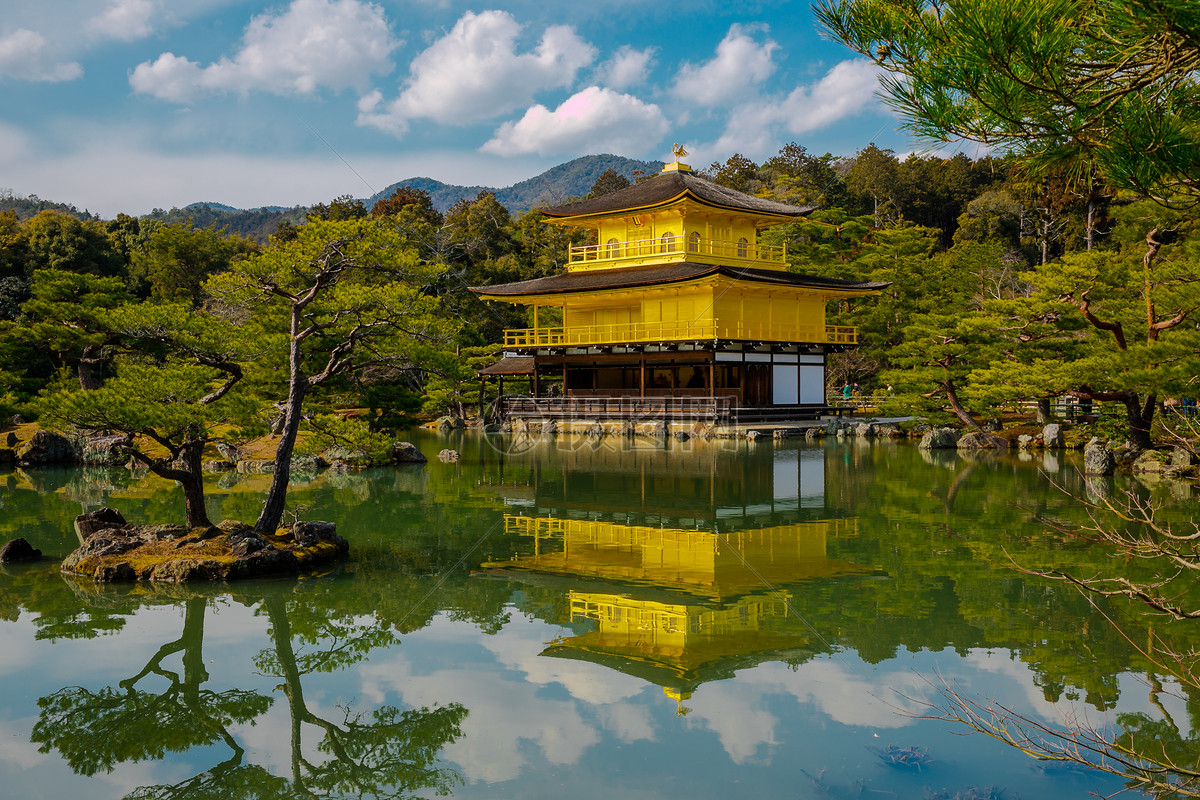
\includegraphics[width=0.9\textwidth]{figure/pic1_source.jpg}
			\end{subfigure}
			\begin{subfigure}{0.36\linewidth}
				\centering
				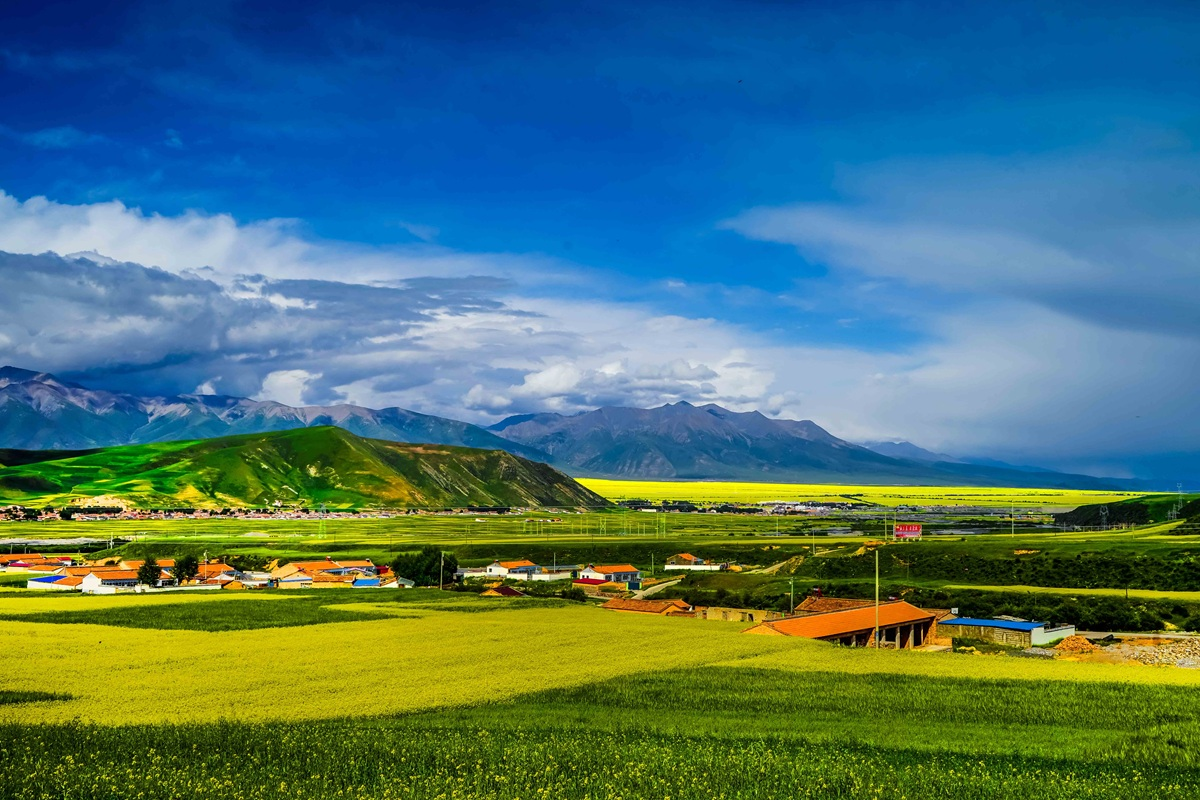
\includegraphics[width=0.9\textwidth]{figure/pic2_source.jpg}
			\end{subfigure}
			\caption{原始图像}
		\end{figure}

		\begin{figure}[htbp]
			\centering
			\begin{subfigure}{0.33\linewidth}
				\centering
				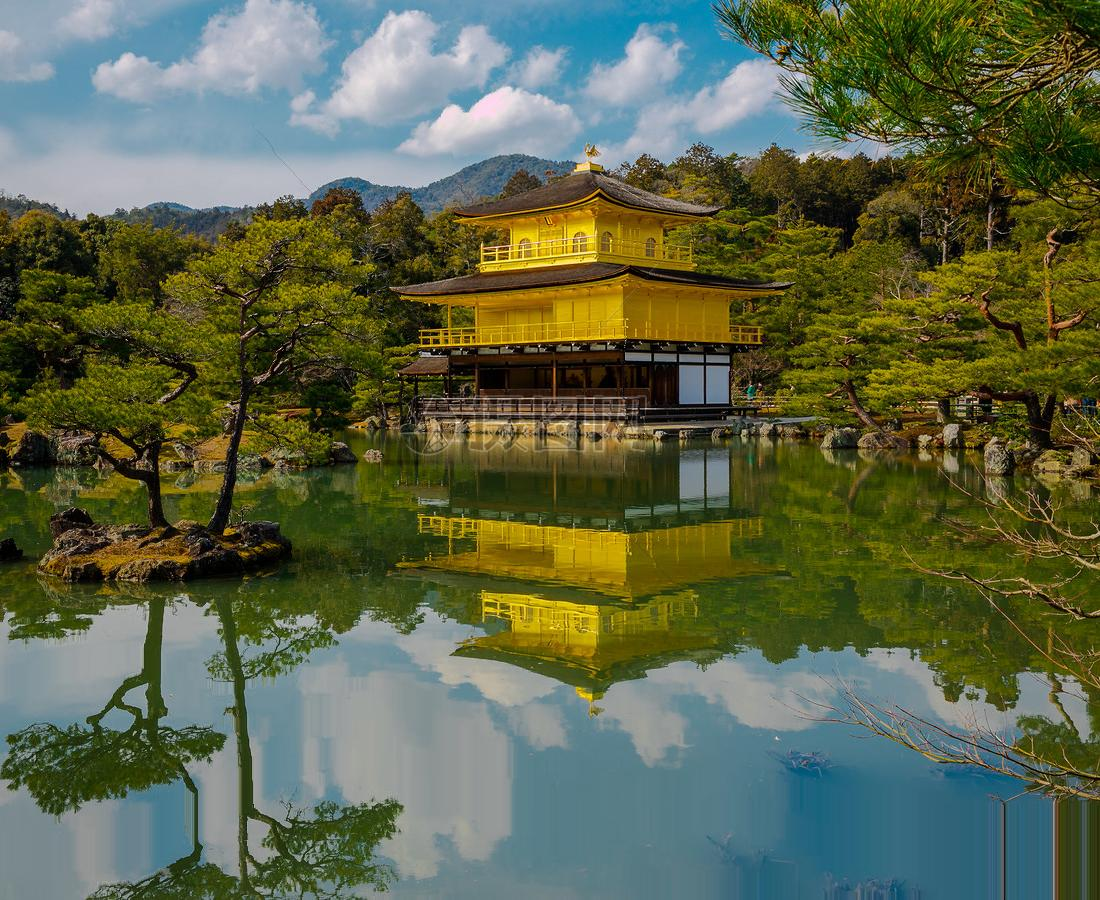
\includegraphics[width=0.9\textwidth]{figure/pic1_result_back.jpg}
			\end{subfigure}
			\begin{subfigure}{0.33\linewidth}
				\centering
				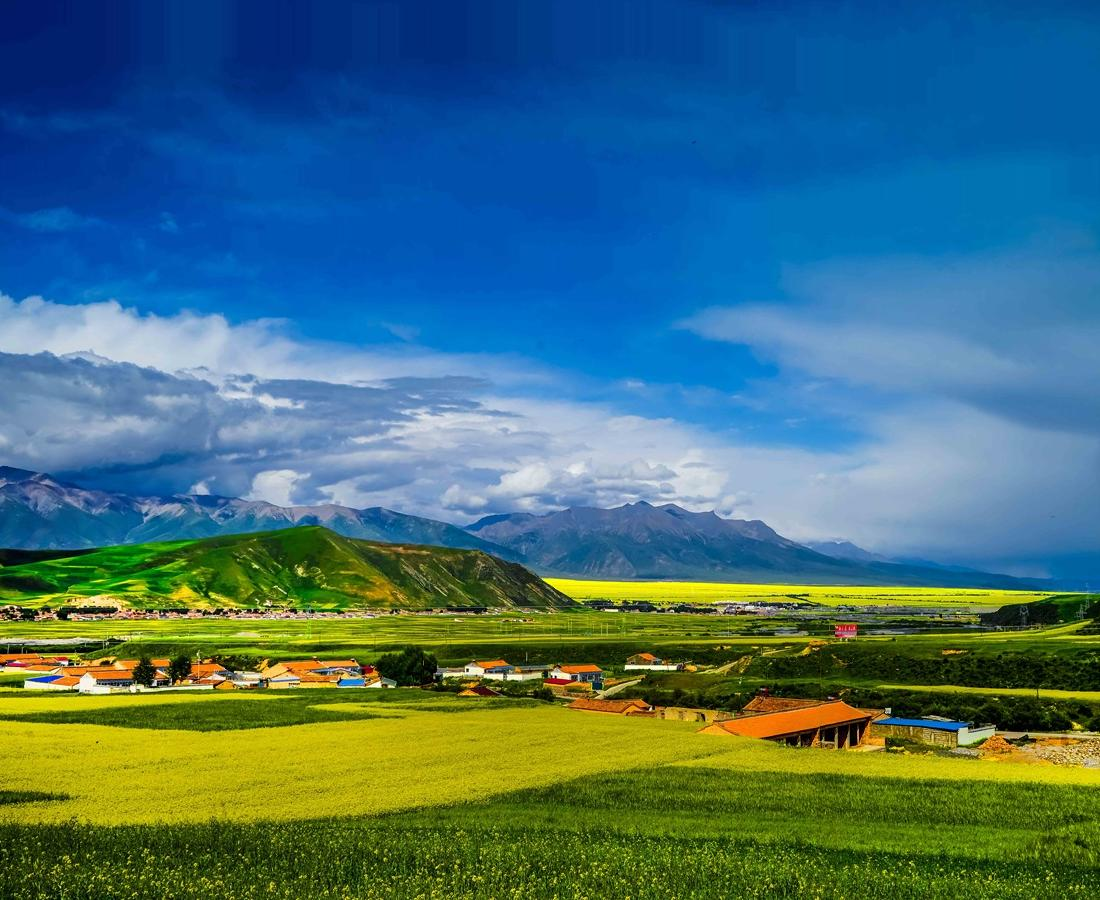
\includegraphics[width=0.9\textwidth]{figure/pic2_result_back.jpg}
			\end{subfigure}
			\caption{从最后一行开始回溯}
		\end{figure}

		\begin{figure}[htbp]
			\centering
			\begin{subfigure}{0.33\linewidth}
				\centering
				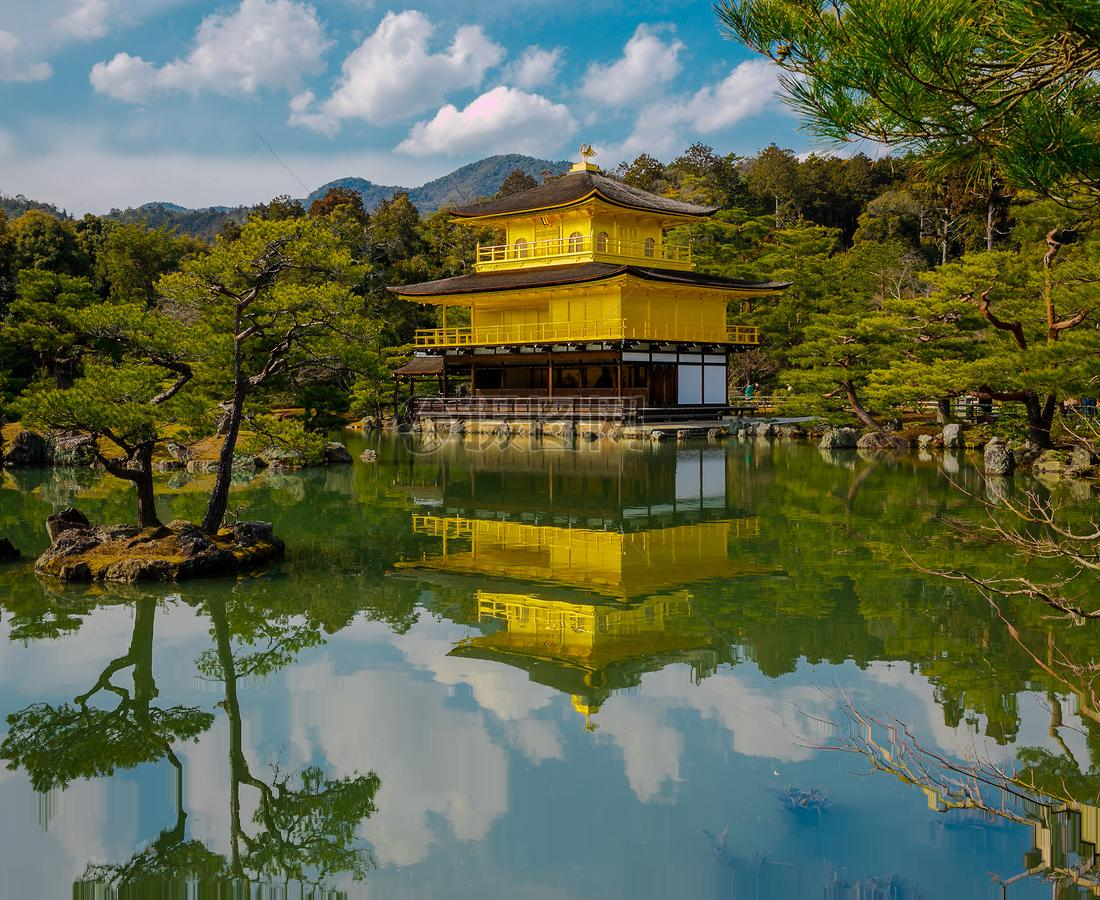
\includegraphics[width=0.9\textwidth]{figure/pic1_result_rand.jpg}
			\end{subfigure}
			\begin{subfigure}{0.33\linewidth}
				\centering
				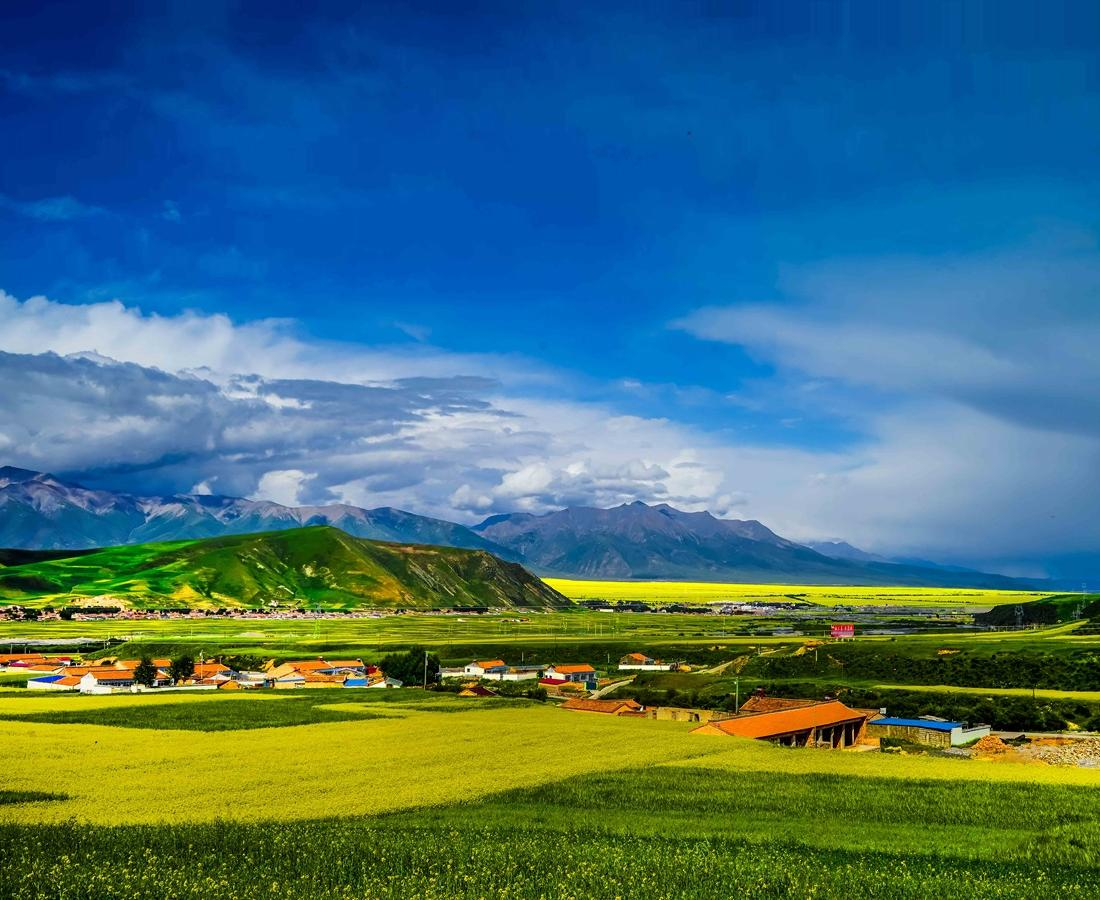
\includegraphics[width=0.9\textwidth]{figure/pic2_result_rand.jpg}
			\end{subfigure}
			\caption{随机选择起始行延申}
		\end{figure}

		\noindent
		从上述结果可以看出, 随机选择起始行的方法在接缝路径的分布上更加均匀 (尤其是左图的右下角处), 图像内容保留更完整, 视觉效果更佳.

		\section{结论}
		\noindent
		本文实现了基于 Seam Carving 的图像缩放算法, 并比较了两种起始行选择策略. 实验结果表明, 随机选择起始行的方法在保持图像内容完整性的同时, 提供了更自然和均匀的缩放效果. 未来的工作可以进一步优化算法, 引入更多的内容感知策略, 以提高图像缩放的质量和效率.

\end{document}
